% !TEX encoding = UTF-8
% !TEX TS-program = pdflatex
% !TEX root = computabilità e algoritmi.tex
% !TEX spellcheck = it-IT

\subsubsection{Codice dell'algoritmo}\label{codice-dellalgoritmo}


\begin{breakablealgorithm}
	\caption{BM: Pattern matching con BoyerMoore}
	\begin{algorithmic}[1]
	\Function{BoyerMoore}{$ P,T $}
	    \State $ pref \gets \text{\textsc{FunzionePrefisso}}(P_{rev}) $
	    \State // parto dal secondo insieme perché è quello che contiene i valori maggiori
	    \For{$ j = m \text{ downto } 0 $}
	        \If{$ j = m - pref[i+1] $}
	            \State $ h \gets j $
	        \EndIf
	        \State // $ h $ è il minimo valore tale che $ max(1,j) \leq h \leq m $ e $ h = m -\pi_{1+h}^{rev} $
	        \State $ d[j] \gets j $
	    \EndFor
	    \State // $ d[j] $ è il minimo del secondo insieme
	    \For{$ h = m \text{ downto } 1 $}
	        \State $ j \gets m - pref[i+h] $
	        \If $  h < j $
	            \State $ d[j] \gets h  $
	       \EndIf
	    \EndFor
	    \State $ i \gets 0 $
	    \While{$ i \leq n - m $}
	        \State $ j \gets m $
	        \While{$ P[j] = T[i+j] $}
	           \State $ j \gets j - 1 $
	        \EndWhile
	        \If{$ j = 0 $}
	            \State Segnala l'occorrenza in posizione $ i + 1 $
	        \EndIf
	        \State $ i \gets i + d[j] $
	      \EndWhile
	  \EndFunction
	  \end{algorithmic}
\end{breakablealgorithm}

\subsubsection{Complessità}\label{complessituxe0}

La pre-elaborazione richiede \emph{O(3m)}, mentre la dimostrazione che il
tempo richiesto è lineare è complessa e non viene affrontata. Nel caso
pessimo, la fase di ricerca fa \emph{O(4n)} confronti.

Questo algoritmo risulta comunque molto utilizzato in pratica, perché il
più delle volte vengono fatti meno di \emph{n} confronti.

Ad esempio, supponendo di avere un pattern che inizia con un carattere,
che compare solo all'inizio e trovando un mismatch sul secondo
carattere, si ha uno spostamento di \emph{m} con solamente due
confronti.

Questo perché se il primo carattere matcha con la stringa e non
ricompare mai all'interno del pattern, l'unico modo per avere un match
completo è quello di spostarsi di \emph{m}.

\subsection{Knuth, Morris e Pratt on-line}\label{knuth-morris-e-pratt-on-line}

Versione dell'algoritmo \textsc{KMP} che funziona controllando esattamente una volta ogni carattere del testo. Per poter applicare l'algoritmo è necessario che l'alfabeto $ \Sigma $ sia finito e noto a
priori.

Supponiamo che il pattern sia allineato nella posizione \textit{j} del testo e che i primi $j-1$ caratteri del pattern siano stati trovati uguali a quelli del testo.

Sia $ k =i+j-1 $ la posizione del testo allineata con la posizione \textit{j} del pattern. Si ha quindi che 

$$
P[1, j-1] = T[i, k-1]
$$

Supponiamo poi che ci sia un'altra occorrenza del pattern in una posizione $ i+h $ del testo compresa tra $ i$ e $ i+j-1 $.

Se questo è vero si ha che 

$$
P[1, j-h] = T[i+h,k]
$$

Siccome $ P[1,j-1] = T[i , k-1] $ dovrà essere

$$
P[1, j-h-1] = T[i+h, k-1] = P[1+h, j-1] \text{ e } P[j-h] = T[k]
$$

Ovvero dal carattere $ 1+h $ del pattern inizia un prefisso del pattern di lunghezza $ j -h -1 $.

\begin{figure}[htbp]
	\centering
	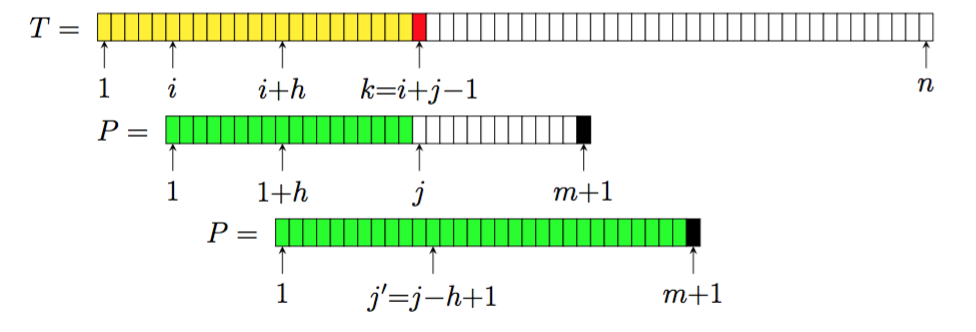
\includegraphics[width=0.9\textwidth]{./notes/immagini/l14-fig1}
\end{figure}

Pertanto, la prima posizione del testo compresa tra \textit{i} e $ k = i + h -1 $  in cui può esserci una occorrenza del pattern è la prima posizione $ i+h $ tale che:

$$
\underbrace{P[1, j -h -1] = P[1+h, j -1]}_{\text{prefisso a partire da $ 1+h $}} \text{ e } \underbrace{P[j-h] = T[k]}_{\text{carattere corrente uguale}}
$$

Se $ T[k] = P[j] $, ovvero $ h=0 $, si ha che la prima posizione da cui può partire un match completo è $ i $.

Se $ T[k] \neq P[j] $ allora $ i+h $ è la prima posizione in cui valgono le condizioni sopra riportate, ovvero che $ \pi_{1+h}^P = j - h -1 $ e $ P[j-h] = T[k] $.

Se non è possibile trovare un $ h $ compreso tra $ 0 $ e $ j-1 $ ($ i \leq h \leq i+j-1 $), allora la prima posizione del testo in cui può esserci una occorrenza del pattern è $ i+j $.

Pertanto lo spostamento del pattern in funzione di $ j = 1, \ldots, m +1 $ e del carattere $ T[k] = x $ è uguale a 0 se $ P[j] = x $, altrimenti è 

$$
h(j,x) = \min(\{j\} \cup \{h | 0 < h < j, j = 1+h + \pi_{1+h}^P, \: \underbrace{P[ 1+ \pi_{1+h}^P] = x}_{P[j-h] = T[k]}\})
$$

Se l'alfabeto è finito e noto a priori è possibile calcolare in fase di pre-elaborazione del pattern lo spostamento $ h(j,x) $ per ogni carattere dell'alfabeto e per ogni $ j $.
Inoltre, dato che dopo lo spostamento o il pattern è allineato sul carattere successivo a $ T[k] $ (spostamento pari a $ j $) oppure $ T[k] $ è uguale al carattere $ P[j-h] $ del pattern, è possibile passare a confrontare il carattere successivo $ T[k+1] $ il quale risulta essere allineato a $ P[j-h+1] $.
 
Per ogni carattere del testo l'algoritmo sposta il pattern di una quantità $ h $ (che può anche essere 0) che dipende dal carattere stesso e dalla posizione \textit{j} del carattere del pattern che è allineato con il carattere del testo considerato.

Quindi l'unica informazione che serve all'algoritmo per effettuare il passo successivo è la posizione $ j' = j - h+ 1 $ del carattere del pattern che risulterà allineato con il carattere $ T[k+1] $ del testo dopo lo spostamento. Pertanto durante la pre-elaborazione conviene calcolare $ \delta(j,x) $ piuttosto che $ h(j,x) $

$$
\delta(j,x) = j - h(j,x)+1
$$

Che per ogni carattere del pattern e per ogni possibile carattere dell'alfabeto restituisce la posizione $ j' $ del carattere del pattern che risulterà essere allineato con il carattere del testo $ T[k+1] $ dopo lo spostamento relativo al caso $ T[k] = x $.

Se $ j' =m+1 $ si ha che $ P[1,m] = T[k-m+1,k] $, ovvero c'è un'occorrenza del pattern a partire dalla posizione $ k -m+1 $.

Osserviamo che $ \delta(j,x) $ è anche la lunghezza del più lungo suffisso di $ P[1,j-1]x $ che è anche prefisso di $ P $ aumentata di 1.

$$
\delta(j,x) = \begin{cases}
j+1 & \text{ se } P[j] = x \\
\max(\{1\} \cup \{ j - h + 1 | 0 < h < j, \: j = 1 + h + \pi_{1+h}^P, \: P[j-h] = x\}) & \text{ altrimenti}
\end{cases}
$$

\subsubsection{Algoritmo}

\begin{breakablealgorithm}
	\caption{KMP-Online: Algoritmo di Knuth-Morris-Pratt online}
	\begin{algorithmic}[1]
		\Function{KnuthMorrisPrattOnLine}{$ P, T, \Sigma $}
			\State $ pref \gets $ \textsc{FunzionePrefisso}$ (P) $
			\For{$ j=1 \text{ to } m+1 $}
				\For{$ \forall x \in \Sigma $}
					\State $ \delta(j,x) \gets 1 $
				\EndFor
			\EndFor
			\For{$ j=1 \text{ to } m $}
				\State $ \delta(j, P[j]) \gets j+1 $ \Comment{Caso $ P[j] = x = T[k] $}
			\EndFor
			\For{$ h = m \text{ downto } 1$} \Comment{Ciclo al contrario per ottenere il massimo}
				\State $ j \gets 1 + h + pref[1 + h] $
				\State $ \delta(j, P[j-h]) \gets j -h +1  $
			\EndFor
			\State $ j \gets 1 $
			\For{$ k = 1 \text{ to } n$}
				\State $ j \gets \delta(j, T[k]) $
				\If{$ j = m+1 $}
					\State occorrenza in $ k-m+1 $
				\EndIf
			\EndFor
		\EndFunction
	\end{algorithmic}
\end{breakablealgorithm}


La fase di pre-elaborazione ha complessità $ O(m \cdot | \Sigma|) $ mentre la ricerca ha complessità $ O(n) $, ottenendo una complessità totale dell'algoritmo pari a $ O(m + n) $.

\subsubsection{$ \delta $ come automa a stati finiti}

\todo[inline]{TODO}

L'algoritmo si comporta come un'automa a stati finiti...

Dalla tabella (inserire tabella) si può ottenere il grafo (inserire grafo)

\subsection{Algoritmo di Aho Corasick}\label{algoritmo-di-aho-corasick}

Algoritmo che funziona in modo simile a KNP-online, con la differenza
che permette di effettuare il pattern matching utilizzando più pattern
contemporaneamente.
